%% ****** Start of file apstemplate.tex ****** %
%% %%
%% %%%%
%%   This file is part of the APS files in the REVTeX 4.2 distribution.
%%   Version 4.2a of REVTeX, January, 2015
%% %%
%% %%%%
%%   Copyright (c) 2015 The American Physical Society.
%% %%
%%   See the REVTeX 4 README file for restrictions and more information.
%% %%
%% %%%
% This is a template for producing manuscripts for use with REVTEX 4.2
% Copy this file to another name and then work on that file. That way,
% you always have this original template file to use.
% %
% Group addresses by affiliation; use superscriptaddress for long author
% lists, or if there are many overlapping affiliations. For Phys. Rev.
% appearance, change preprint to twocolumn. Choose pra, prb, prc, prd,
% pre, prl, prstab, prstper, or rmp for journal Add 'draft' option to
% mark overfull boxes with black boxes Add 'showkeys' option to make
% keywords appear
%\documentclass[aps,prstab,groupedaddress,reprint]{revtex4-2} % from
%lance
\documentclass[% 
reprint, superscriptaddress,
%groupedaddress, unsortedaddress, runinaddress, frontmatterverbose,
%preprint, preprintnumbers, nofootinbib, nobibnotes, bibnotes,
 amsmath,amssymb, aps,
%pra, prb, rmp,
prstab,
%prstper, floatfix,
]{revtex4-2}
\usepackage{graphicx} \usepackage{float}
\usepackage[caption=false]{subfig}
%\usepackage[font=footnotesize]{caption}
%\usepackage[font=footnotesize]{subcaption}
\usepackage{wrapfig} \usepackage{lipsum} \usepackage{mathtools}
\usepackage{mathrsfs} \usepackage{amsfonts} \usepackage{enumitem}
\usepackage{amsmath} \usepackage{amssymb}
%\usepackage[margin=0.8in]{geometry}
\usepackage[dvipsnames]{color} \usepackage{epstopdf} \usepackage{braket}
\usepackage{verbatim}
%\documentclass[aps,prl,preprint,superscriptaddress]{revtex4-2}
%\documentclass[aps,prl,reprint,groupedaddress]{revtex4-2}
%
% You should use BibTeX and apsrev.bst for references Choosing a journal
% automatically selects the correct APS BibTeX style file (bst file), so
% only uncomment the line below if necessary.
%\bibliographystyle{apsrev4-2}
%
% In order to include 2 by 2 figures
%\usepackage{subfig}

\begin{document}

% Use the \preprint command to place your local institutional report
% number in the upper righthand corner of the title page in preprint
% mode. Multiple \preprint commands are allowed. Use the
% 'preprintnumbers' class option to override journal defaults to display
% numbers if necessary
%\preprint{}
%
%Title of paper
\title{Emittance Preservation Through Density Ramp Matching Sections in a Plasma
Wakefield Accelerator} \author{Yujian Zhao}
%\email[]{zhaoyujian@ucla.edu}
\affiliation{Department of Physics and Astronomy, University of
California Los Angeles, Los Angeles, CA 90095, USA}
% repeat the \author .. \affiliation  etc. as needed \email, \thanks,
% \homepage, \altaffiliation all apply to the current author.
% Explanatory text should go in the []'s, actual e-mail address or url
% should go in the {}'s for \email and \homepage. Please use the
% appropriate macro foreach each type of information
% 
% \affiliation command applies to all authors since the last
% \affiliation command. The \affiliation command should follow the other
% information \affiliation can be followed by \email, \homepage, \thanks
% as well.
% 
%\author{Y. Zhao\textsuperscript{1}, W. An\textsuperscript{1}, X.
%Xu\textsuperscript{1},L. Hildebrand\textsuperscript{1},  M. J.
%Hogan\textsuperscript{2}, V. Yakimenko\textsuperscript{2}, C.
%Joshi\textsuperscript{1}, W. B. Mori\textsuperscript{1}\\
%\textsuperscript{1}\textit{University of California, Los Angeles,
%California 90095, USA}\\ \textsuperscript{2}\textit{SLAC National
%Accelerator Laboratory, Menlo Park, California 94025, USA}}
%
\author{Weiming An} \email{anweiming@bnu.edu.cn} 
\affiliation{Department of Astronomy, Beijing Normal University, Beijing 100875, China}
\affiliation{Department
of Physics and Astronomy, University of California Los Angeles, Los
Angeles, CA 90095, USA}

\author{Xinlu Xu} \email{xuxinlu04@gmail.com} \affiliation{Department of
Physics and Astronomy, University of California Los Angeles, Los
Angeles, CA 90095, USA} \affiliation{SLAC National Accelerator
Laboratory, Menlo Park, California 94025, USA}

\author{Fei Li} \affiliation{Department of Physics and
Astronomy, University of California Los Angeles, Los Angeles, CA 90095,
USA}

\author{Lance Hildebrand} \affiliation{Department of Physics and
Astronomy, University of California Los Angeles, Los Angeles, CA 90095,
USA}

\author{Mark J. Hogan} \affiliation{SLAC National Accelerator
Laboratory, Menlo Park, California 94025, USA} \author{Vitaly Yakimenko}
\affiliation{SLAC National Accelerator Laboratory, Menlo Park,
California 94025, USA} \author{Chan Joshi} \affiliation{Department of
Electrical Engineering, University of California Los Angeles, Los
Angeles, CA 90095, USA} \author{Warren B. Mori} \affiliation{Department
of Physics and Astronomy, University of California Los Angeles, Los
Angeles, CA 90095, USA} \affiliation{Department of Electrical
Engineering, University of California Los Angeles, Los Angeles, CA
90095, USA}



%\homepage[]{Your web page} \thanks{} \altaffiliation{} \affiliation{}
%
%Collaboration name if desired (requires use of superscriptaddress
%option in \documentclass). \noaffiliation is required (may also be used
%with the \author command). \collaboration can be followed by \email,
%\homepage, \thanks as well. \collaboration{} \noaffiliation
%
\date{\today}

\begin{abstract} In plasma wakefield acceleration, the witness
beam's emittance needs to be preserved when it propagates through a plasma stage. The plasma includes
 density ramps at both the entrance and the exit. Using the
WKB solution of a single particle's motion,  analytical expressions for
the evolution of the beam emittance and the Twiss parameters in an arbitrary adiabatic plasma profile are
provided neglecting the acceleration of the beam inside the plasma. It is
shown that the beam emittance can be preserved under the matching
condition even when the beam has an initial energy spread. It is also shown that the emittance growth for an unmatched beam is minimized when it is focused to the same vacuum plane for a matched beam.  The emittance
evolution from 3D QuickPIC simulation results agree well with the
theoretical results.  
In the some of the proposed experiments on nearly completed FACET II facility, the matching
condition may not be perfectly satisfied and the wake may not be perfectly symmetric. It is shown that for a given set of beam
parameters that are consistent with FACET II capabilities, even when the assumptions of the theory are not satisfied, 
the emittance growth can still be minimized by choosing the optimal focal
plane. Last, another issue that may cause emittance 
growth in realistic plasmas is also examined. When using a lithium plasma source in FACET II experiments a helium buffer gas is used. The plasma is formed from field ionization which can lead to a nonlinear
focusing force when there are
nonuniform helium ions due to its high ionization potential. For an initial beam
emittance of $20 \mathrm{\mu m}$, the
helium ionization is found to be small and the witness beam's emittance can
be preserved. \end{abstract}

% insert suggested keywords - APS authors don't need to do this
%\keywords{}
%
%\maketitle must follow title, authors, abstract, and keywords
\maketitle

% body of paper here - Use proper section commands References should be
% done using the \cite, \ref, and \label commands  WeiLu2006
\section{Introduction} During the past two decades of research, a number of impressive advances have been made in the beam-driven Plasma Wakefield Acceleration (PWFA)  concept. For instance, experiments have shown that these wakes can
sustain accelerating gradients exceeding 50 GeV/m over $\sim$ meter in length
\cite{PWFA2007}, and the acceleration of the witness beam in PWFA
can be highly efficient while maintaining a high acceleration gradient
and small energy spread \cite{PWFA2014}. In PWFA, an ultra-relativistic
electron beam (the drive beam) is used to form a plasma wake 
that accelerates a second electron beam (the witness beam) that is properly loaded inside
the wake. In the so-called blowout regime, the drive beam density is
much higher than the plasma density. The electric field of the drive
beam will expel all the plasma electrons away and leave an
ion channel (i.e. a bubble) after it. As shown in Fig.
\ref{fig:TwoBunches}, when the witness beam is located at a proper
position inside the wake, the accelerating field can be flattened in
order to preserve the energy spread. \begin{figure}[htbp] \centering
\includegraphics[width=0.9\linewidth]{TwoBunches2.png} \caption{A
snapshot of the drive and witness beam of a sample simulation of a two bunch PWFA. A data is in the $x-\xi$ plane at $y=0$.  Both beams (blue) are
propagating to the left. The green area shows the unperturbed plasma electron
density, the white area is the uniform plasma ions (ion channel/bubble).
The red curve is the lineout of the accelerating field $E_z$ on the
axis (in arbitrary units).} \label{fig:TwoBunches} \end{figure} At the back of the bubble,
where the witness beam is located, not only is there a longitudinal
electric field that provides a high acceleration gradient, but there is also a
transverse focusing force. In addition, when
there is azimuthal symmetry, in these nonlinear wakes the longitudinal electric field (the
accelerating field) does not depend on $r$ and the transverse focusing
force is linear (proportional to $r$), points radially inward, and does not depend on $\xi = ct- z$ inside the bubble \cite{WeiLu2006}. The fact that the accelerating field does not depend on $r$ ensures that the beam particles will not gain additional slice energy spread when undergoing acceleration and betatron oscillations inside the bubble. Furthermore, the fact that the transverse linear focusing force does not depend on $\xi$ ensures that the beam particles at different longitudinal positions will oscillate at the same betatron frequency, if they have the same energy. If one of these properties is satisfied then the Panofsky Wenzel theorem \cite{PWT1,PWT} guarantees that the other is as well.

When the beam has no energy spread, its emittance is conserved under a
linear focusing force inside the symmetric bubble. When the beam has an energy
spread, %which may either be an initial one or grow up during the
and/or there is acceleration with imperfect beam loading (particles at different
longitudinal positions in the beam feel a different accelerating field,
$E_z$), the beam's emittance may increase during its propagation in the
plasma. 
% Add the references %%%
The topic of emittance growth and preservation  is very important and is being actively studied
 \cite{Mehrling2012,Dornmair,Antici,Migliorati,Xinlu2016,German2018,German2014,Robert}. 

%%%


Recently, expressions for emittance evolution in uniform plasma, 
both for cases when the beam does \cite{Xinlu2016} or does not have \cite{German2018}
longitudinal acceleration have been published. It has also been shown that several plasma density profiles provide 
exact solutions to single particle motion \cite{Xinlu2016,German2014}, therefore
the evolution of the beam's Twiss parameters can be calculated and used to match the beam into a plasma.
In this paper,  we investigate how the emittance grows when a beam is not matched in an adiabatic plasma ramp.
In complimentary work, R. Ariniello et al. \cite{Robert} have recently shown that if a beam is matched to an adiabatic plasma profile, the emittance will oscillate around its initial value
with a small amplitude ($10^{-4}$ times the initial emittance) for a 2\% energy spread(and the amplitude of oscillations scales as $\sigma_\gamma^2$). 
%Recent works have shown that a particular plasma density ramp
%can be chosen to match the witness beam from an initial spot size to a
%desired spot size with negligible emittance growth \cite{Xinlu2016} and
%how beam emittance evolves in a longitudinally uniform plasma
%\cite{German2018}. 


In typical experiments (e.g. the FACET II experiments at
SLAC \cite{PWFA_FACETII}), the plasma density profile is usually fixed
with density ramps at the entrance and the exit. Therefore the beam parameters need to be optimized to match the beam to the plasma. It has been shown
that if the witness beam is initially matched to the plasma, its
emittance can be preserved very well \cite{PWFA_FACETII}. However, if
the witness beam parameters are fixed, it usually cannot be perfectly matched to an arbitrary plasma density ramp. In this paper, we investigate the witness
beam's emittance evolution in this situation. We first derive an
analytical expression for the beam's emittance evolution in an arbitrary
adiabatic plasma profile, assuming the beam has no longitudinal
acceleration. This analytical expression can be used to predict the
emittance growth when the beam has an energy spread and is not initially matched. This analysis is complimentary to that in \cite{Robert} where it was assumed that the beam was nearly matched and the emittance growth was small. 
We also discuss how to choose the relative focal plane by either moving the plasma or the focal position of the beam to minimize the emittance growth for an
unmatched beam with fixed parameters. It is found that the beam emittance growth can be minimized
when choosing the focal plane to be the vacuum focus for a beam that was matched.
Another issue that may cause emittance growth in recently proposed energy doubling of the witness beam experiment at FACET II experiments \cite{PWFA2007} is the
ionization of helium buffer gas when using the Lithium plasma source. Additional self-ionization \cite{Bruhwiler} by the beam can modify the focusing fields in the buffer region. In the last section, we show that
under that situation the emittance growth is due to the nonlinear
focusing force felt by the beam, which is caused by the nonuniform
helium ion density in the plasma. 
The helium ionization can be minimized by using a 20 $\mathrm{\mu m}$ initial emittance witness bunch. Therefore such a bunch can be propagated while gaining energy without measurable emittance growth.




\section{Theoretical analysis of emittance evolution in arbitrary
adiabatic plasma density profile} In the blowout regime of PWFA with the
assumption of azimuthal symmetry (we will henceforth use this assumption),
the focusing force felt by an electron in the witness beam is
$\textbf{F}_{\perp} = -m_e\omega_p^2\textbf{r}/2$ (where $m_e$ is the electron mass,
$\omega_p =\sqrt{\frac{n_pe^2}{\epsilon_0 m_e}}$ is the plasma frequency, $n_p$ is the plasma density, $\epsilon_0$ is the vacuum permittivity, $e$ is the elementary charge), which is proportional to the radial
distance $r$ and independent of $\xi = ct - z$. Therefore the motions of
the beam particle in $x$ and $y$ directions are decoupled, and we will
only study the beam particle motion in the $x$ direction. If we assume a
beam particle's energy is a constant, the equation of motion for this
particle is \begin{equation} x''(z)  + k_{\beta}(z)^2 x(z) = 0  \label{EOM} \end{equation} 
where $z$ is the coordinate
along the direction of propagation, $k_{\beta}(z) = \frac{\omega_p(z)}{\sqrt{2\gamma}
c}$,  $\omega_p(z)$ is the plasma frequency at position
$z$, $\gamma$ is the relativistic factor of
the beam particle, $c$ is the speed of light. In a uniform plasma, $\omega_p(z)$ is a constant, so the solution to
equation (\ref{EOM}) is a simple harmonic oscillation. With a given
initial phase space distribution for the beam, we can obtain an analytical
expression for the emittance evolution\cite{Xinlu2016,German2018}.
For nonuniform plasma, there is no general analytical solution to
equation (\ref{EOM}). However, as long as the plasma density is changing
adiabatically, i.e., 
\begin{equation}
\frac{|k'_{\beta}(z)| \frac{2\pi}{k_{\beta}(z)} }{k_{\beta}(z)} \ll 1
\label{adiabatic_condition} 
\end{equation}
or 
\[
	\frac{\pi}{k_{\beta}(z)n_p(z)} \left|\frac{dn_p(z)}{dz}\right| \ll 1
\]
 we can use WKB method \cite{Griffiths} to get an approximate
solution to equation (\ref{EOM}), and calculate the emittance evolution
with the WKB solution.

The WKB solution to equation (\ref{EOM}) is: \begin{equation}
\begin{aligned} x(z)& = x(0)
\frac{\sqrt{\beta_{m}(z)}}{\sqrt{\beta_{m}(0)}}\cos[\phi(z)]\\
&+\sqrt{\beta_{m}(z)\beta_{m}(0)}\Big[ x'(0) +
\frac{\alpha_m(0)}{\beta_m(0)}x(0)\Big]\sin[\phi(z)] \end{aligned}
\label{WKB} \end{equation} where 
\begin{equation}
\beta_m(z) = 1/k_{\beta}(z),\; \alpha_m(z) =
-\frac{1}{2}\frac{d\beta_m(z)}{dz}
\label{matchedAlphaBeta}
\end{equation}
are the Twiss parameters for a single particle in an adiabatically changing profile, 
and $\phi(z) = \int_{0}^{z}
k_{\beta}(s) ds$ is the phase advance. $x(0)$ and $x'(0)$ are the initial values for
the beam particle. Then the adiabatic condition (\ref{adiabatic_condition}) can be simplified to \cite{Robert}
 \begin{equation}
 |\alpha_m(z)| \ll 1
 \label{adiabatic_condition_alpha}
 \end{equation}
We note that if the plasma density profile is $n_p(z)
= \frac{n_{p0}}{(1+z/l)^4}$ (where $l$ is a constant), then equation
(\ref{EOM}) has an exact solution \cite{German2014}, which is the same
as its WKB solution described in equation (\ref{WKB}).

For brevity, we henceforth denote $x(z)$ by $x$, $x(0)$ by $x_i$, 
$\beta_m(z)$ by $\beta_{m}$, $\beta_m(0)$ by $\beta_{mi}$, 
$\alpha_m(z)$ by $\alpha_{m}$, $\alpha_m(0)$ by $\alpha_{mi}$, $\phi(z)$ by $\phi$.
From (\ref{WKB}) and its derivative, we can obtain \[ \begin{pmatrix} x \\ x'
\end{pmatrix} = M \begin{pmatrix} x_i \\ x'_i \end{pmatrix} =
\begin{pmatrix} M_{11} & M_{12} \\ M_{21} & M_{22} \end{pmatrix}
\begin{pmatrix} x_i \\ x'_i \end{pmatrix} \] where $M$ is the
transport matrix and \[ \begin{aligned} M_{11} &=
\sqrt{\frac{\beta_m}{\beta_{mi}}}(\cos \phi + \alpha_{mi}\sin \phi)
\\ M_{12} &= \sqrt{\beta_m\beta_{mi}}\sin \phi \\ M_{21} &=
\frac{(\alpha_{mi}-\alpha_m)\cos \phi -
(1+\alpha_{mi}\alpha_m)\sin \phi}{\sqrt{\beta_m\beta_{mi}}} \\
M_{22} &= \sqrt{\frac{\beta_{mi}}{\beta_m}}(\cos \phi -
\alpha_m\sin \phi) \end{aligned} \]

The geometric emittance is defined as 
\begin{equation}
 \epsilon = \sqrt{\braket{x^2}\braket{x'^2}-\braket{xx'}^2 } 
 \label{geoEmittanceDef}
\end {equation}
where
$\braket{}$ is the ensemble average. It then follows that (see Appendix A
for details) \begin{equation} \begin{aligned} \braket{x^2} &=
\braket{(M_{11}x_i + M_{12}x'_i)^2 } \\ &= \epsilon_i\beta_m(A +
B_1 C + B_2S) , \end{aligned}\label{x2} \end{equation} where: \[
\begin{aligned} A &= \frac{\beta_i \gamma_{mi}+\gamma_i
\beta_{mi}-2\alpha_i \alpha_{mi}}{2}, \\ B_1 &=
\frac{\beta_i}{\beta_{mi}} - A = \frac{\beta_i}{\beta_{mi}}
-\frac{\beta_i \gamma_{mi}+\gamma_i \beta_{mi}-2\alpha_i
\alpha_{mi}}{2}, \\ B_2 &= \frac{\beta_i}{\beta_{mi}}\alpha_{mi}-\alpha_i,
\\ C &= \int d\phi f_\phi(\phi)\cos 2\phi , \\ S & = \int d\phi
f_\phi(\phi)\sin 2\phi, \end{aligned} \] and $\epsilon_i =
\sqrt{\braket{x_i^2}\braket{{x'_i}^2}-\braket{x_ix'_i}^2}$, $\beta_i =
\braket{{x_i}^2}/\epsilon_i$, $\gamma_i = \braket{{x'_i}^2}/\epsilon_i$,
$\alpha_i = -\braket{x_ix'_i}/\epsilon_i$ are the beam's initial geometric emittance and Twiss parameters, $\gamma_m =
(1+\alpha_m^2)/\beta_m$, and $f_\phi(\phi)$ is the 
distribution function for the beam particles' phase advance. For a beam with no energy spread, $f_\phi(\phi) = \delta (\phi - \phi_0)$ 
where $\phi_0 = \int_{0}^{z} k_{\beta}(s) ds =\int_{0}^{z} \frac{\omega_p(s)}{\sqrt{2 \gamma}c} ds$.

We can also obtain 

\begin{equation}
\begin{aligned} \braket{x'^2} = \epsilon_i \Big[&A
\gamma_m+\frac{-B_1-2B_2\alpha_m + B_1\alpha_m^2}{\beta_m}C  
\label{x'2} \\ &+\frac{-B_2+2B_1\alpha_m +B_2
\alpha_m^2}{\beta_m}S \Big] 
\end{aligned} 
\end{equation} and


\begin{equation} 
\braket{xx'} = -\epsilon_i
[A\alpha_m +(B_1\alpha_m-B_2)C+(B_2\alpha_m+B_1)S] 
\label{xx'}
\end{equation}

Using equations (\ref{x2})-(\ref{xx'}), and noting that $A$,
$B_1$ and $B_2$ satisfy $B_1^2 + B_2^2 = A^2 -1$, we can obtain an analytical expression of emittance growth for arbitrary $f_\phi(\phi)$ with small energy spread
\begin{equation} \begin{aligned}
\epsilon &= \sqrt{\braket{x^2}\braket{x'^2}-\braket{xx'}^2 } \\
&=\epsilon_i\sqrt{A^2 -(A^2 - 1) (C^2 + S^2)} \\
\label{emittance_general}\end{aligned} \end{equation}


Denote the average relativistic factor of the beam as $\bar{\gamma}$. When the
relative energy spread of the beam is very small (i.e. for every
particle $|\Delta\gamma| = |\gamma-\bar{\gamma}| \ll \bar{\gamma}$), the
particle's phase advance in the plasma $\phi$ will become $
\phi(\gamma) = \bar{\phi} - \frac{\bar{\phi}}{2 \bar \gamma} \Delta
\gamma$, where $\bar{\phi} = \phi(\bar{\gamma})$ (See Appendix C for details). Assuming a Gaussian 
energy distribution, for the beam particles we have:
 \[ f_\gamma(\gamma) = \frac{1}{\sqrt{2\pi}\sigma_\gamma}
\exp[-\frac{(\gamma-\bar \gamma)^2}{2\sigma_\gamma^2}] \] As a result,
$\phi$ will also have a Gaussian distribution \[ f_\phi(\phi) =
\frac{1}{\sqrt{2\pi}\sigma_\phi} \exp[-\frac{(\phi-\bar
\phi)^2}{2\sigma_\phi^2}] \] where 
\begin{equation}
\sigma_\phi = \frac{\bar \phi}{2}
\frac{\sigma_\gamma}{\bar \gamma}
\label{sigmaPhiandSigmaGamma}
\end{equation}
$\frac{\sigma_\gamma}{\bar
\gamma}$ is the relative energy spread of the beam. With this Gaussian
distribution of $\phi$, we can obtain: \begin{equation}
C=\exp(-2\sigma_\phi^2) \cos(2\bar \phi),\;\;S=\exp(-2\sigma_\phi^2)
\sin(2\bar \phi) \label{GaussianCS} \end{equation}

Inserting (\ref{GaussianCS}) into (\ref{emittance_general}) and using (\ref{sigmaPhiandSigmaGamma}), we get an analytical expression of emittance growth for a beam that has a Gaussian energy distribution with a small energy spread:
% \begin{equation} \begin{aligned}
%\epsilon &=\epsilon_i\sqrt{A^2 -(A^2 -1) \exp(-4\sigma_\phi^2)} \\
%&=\epsilon_i\sqrt{A^2 -(A^2 -1) \exp[-(\frac{\sigma_\gamma}{\bar
%\gamma}\bar \phi)^2]}. \end{aligned} \end{equation}  

\begin{equation} \frac{\epsilon}{\epsilon_i}=A\sqrt{ 1-\frac{A^2
-1}{A^2} \exp[-(\frac{\sigma_\gamma}{\bar \gamma}\bar \phi)^2]}  
\label{emittance} \end{equation} where $\frac{\sigma_\gamma}{\bar
\gamma}$ is the energy spread, and $\bar \phi = \frac{1}{\sqrt{2 \bar
\gamma}c}\int_0^z \omega_p(s) ds$ is the phase change of an electron with energy $\bar \gamma$ after it
propagates for a longitudinal distance of $z$ inside the plasma. Because we assume the beam's energy, $\bar \gamma$, does not change, then 
\[
\frac{\epsilon}{\epsilon_i}= \frac{\bar \gamma \epsilon}{\bar \gamma \epsilon_i} \approx \frac{\epsilon_n}{\epsilon_{ni}}
\]
where $\epsilon_n = \frac{1}{m_ec} \sqrt{\braket{x^2}\braket{p_x^2}-\braket{xp_x}^2 }$
is the normalized emittance and $p_x$ is the transverse momentum of the particle. This means the normalized emittance growth is approximately the same as the geometric emittance growth. Note that in order to keep the analysis tractable we have only kept the effects of the energy spread in the betatron phase advance and not on the amplitude of the betatron oscillation in the elements of the transport matrix. The amplitudes are functions of the local values of the Twiss parameters while the phase is an integral in $z$ over $1/\beta_m$. Therefore, only the phase terms can deviate substantially between particles with small energy differences.  Thus, the small amplitude oscillation of the emittance seen in Ref. \cite{Robert} when a matched beam has finite energy spread is absent here.

In Fig. \ref{fig:emittance evolution in ramp}, we compare the
theoretical results from (\ref{emittance}) with QuickPIC \cite{QuickPIC2006,QuickPIC2013}  simulation results. We choose a plasma
density profile $n_p(z) = \frac{n_{p0}}{(1+z/l)^2}$, for which the adiabatic condition is independent of $z$. In the
simulation, we turn off the longitudinal acceleration for the beam
particles (i.e. the energy of the beam particle essentially does not change), and
choose reasonable parameters to make the simulation in the blowout
regime. Fig. \ref{fig:emittance evolution in ramp}(a) shows that when the
beam is initially matched, the beam's emittance is a constant during its
propagation inside the plasma. As shown in Fig. \ref{fig:emittance evolution in ramp}(b)(c)(d), if the beam is not initially matched, the
theoretical results based on the WKB solution agree with the
simulation result very well.


\begin{figure}[!ht]
   \centering
   \subfloat[][]{\includegraphics[width=.23\textwidth]{emittance_in_ramp_match.eps}}\quad
   \subfloat[][]{\includegraphics[width=.23\textwidth]{emittance_scan_energySpread.eps}}\\
   \subfloat[][]{\includegraphics[width=.23\textwidth]{emittance_scan_alpha.eps}}\quad
   \subfloat[][]{\includegraphics[width=.23\textwidth]{emittance_scan_beta.eps}}
   \caption{Emittance evolution in plasma ramp: $n_p(z) =
        \frac{n_{p0}}{(1+z/l)^2}$ $(l = 5$, $l$ and $z$ are normalized
        to $\beta_{mi}$). For (a) the
        beam is initially matched: $\beta_i = \beta_{mi},\;\alpha_i =
        \alpha_{mi} = -\frac{1}{2l} = -0.1 $, and the beam has a 5\% energy spread. For (b) the beam is initially unmatched: $\beta_i
        =10 \beta_{mi},\;\alpha_i =2 \alpha_{mi}$, and the beam has 1\%, 5\%, 10\% initial energy spreads respectively. For (c) the
        beam is initially unmatched: $\beta_i = 10\beta_{mi},\;\alpha_i =
        2\alpha_{mi}, 100\alpha_{mi}, -100\alpha_{mi}$ respectively, and the beam has a 5\% energy spread. For (d) the beam is initially unmatched: $\alpha_i =2 \alpha_{mi}, \; \beta_i
        =5 \beta_{mi},10 \beta_{mi}, 20 \beta_{mi}$ respectively, and the beam has a 5\% energy spread. In (b)(c)(d), the solid lines are from QuickPIC simulations, and the dashed lines are from the analytical expression (\ref{emittance}). In these three plots, the solid black lines correspond to the same simulation result, and the dashed black lines correspond to the same analytical expression.}
   \label{fig:emittance evolution in ramp}
\end{figure}


Note that in (\ref{emittance}), $A \geqslant 1$ is always true (see the Appendix B). So
$\epsilon/\epsilon_i \leqslant A$. When the beam propagates in the
plasma for a very long distance, $\bar \phi$ will become very large, and
the beam will have a saturated emittance: 
\begin{equation}
\frac{\epsilon_{sat}}{\epsilon_i}=A = \frac{\beta_i \gamma_{mi}+\gamma_i \beta_{mi}-2\alpha_i \alpha_{mi}}{2} 
\label{A}
\end{equation}

For the special case when the plasma is uniform along $z$, we have $\alpha_{m} = \alpha_{mi} = 0$, so $\gamma_{m} = \gamma_{mi} = 1 /
\beta_{mi}$, then
\[ A = \frac{\gamma_i \beta_{mi} + \beta_i / \beta_{mi}}{2} \]
Therefore, the emittance growth in a longitudinally uniform plasma will
be 
\begin{equation}
\begin{aligned}
 \frac{\epsilon}{\epsilon_i}=& \frac{\gamma_i \beta_{mi} + \beta_i / \beta_{mi}}{2} \times
 \\
 &\sqrt{1 -\frac{(\gamma_i \beta_{mi} + \beta_i / \beta_{mi})^2-4}{(\gamma_i \beta_{mi} + \beta_i / \beta_{mi})^2}
\exp[-(\frac{\sigma_\gamma}{\bar \gamma}\bar \phi)^2]} 
\label{emittance_uniform}
\end{aligned}
\end{equation}
which is mathematically equivalent to equation (7) in \cite{German2018}, and similar to equation (1) in \cite{Xinlu2016} (difference is due to the different assumptions for $f_\phi(\phi)$).

We define the beam to be initially matched when
\begin{equation}
\alpha_i  = \alpha_{mi} ,\; \beta_i  = \beta_{mi} , \; \gamma_i  = \gamma_{mi} 
\label{match} 
\end{equation} 
Then we have $A = 1, B_1 = 0, B_2 = 0$.
Therefore, from equations (\ref{x2}) - (\ref{xx'}) and
(\ref{emittance}), we have $\braket{x^2}/\epsilon_i = \beta_m$,
$\braket{x'^2}/\epsilon_i = \gamma_m$, $-\braket{xx'}/\epsilon_i =
\alpha_m$ and $\epsilon = \epsilon_i$. So $\beta = \braket{x^2}/\epsilon = \beta_m$, $\gamma = \braket{x'^2}/\epsilon = \gamma_{mi}$, $\alpha = -\braket{xx'}/\epsilon = \alpha_m$.
Therefore, with an
adiabatic plasma density profile, when neglecting the beam's energy
change, if the beam is initially matched, the beam's Twiss parameters
along $z$ will be $\beta_m, \gamma_m, \alpha_m$, and
the beam's geometric emittance will not change. We can therefore interpret $\beta_m$, $\alpha_m$ defined in (\ref{matchedAlphaBeta}) and $\gamma_m$ as the matched Twiss parameters.

If the beam's initial Twiss parameters deviate from the matched ones, i.e.,
\[
\alpha_i  = \alpha_{mi} + \Delta \alpha ,\; \beta_i  = \beta_{mi} + \Delta \beta 
\]
where $|\Delta \alpha | \ll 1$ and $|\Delta \beta| / \beta_{mi} \ll 1$, then
\begin{equation}
A \approx 1 + \frac{1}{2} \Delta \alpha^2 + \frac{\gamma_{mi}}{2\beta_{mi}} \Delta \beta^2 - \frac{\alpha_{mi}}{\beta_{mi}} \Delta \alpha \Delta \beta
\label{deltaA}
\end{equation}

Inserting this into (\ref{emittance}) gives
\[
\frac{\epsilon}{\epsilon_i} \approx 1 +  ( \frac{1}{2} \Delta \alpha^2 + \frac{\gamma_{mi}}{2\beta_{mi}} \Delta \beta^2 - \frac{\alpha_{mi}}{\beta_{mi}} \Delta \alpha \Delta \beta )[1-e^{-(\frac{\sigma_\gamma}{\bar \gamma}\bar \phi)^2}]
\]

We can also get the expression for $\beta$ from the above equations. Inserting (\ref{GaussianCS}) into (\ref{x2}) and using (\ref{sigmaPhiandSigmaGamma}) leads to
\[
\braket{x^2} =\epsilon_i \beta_m \left \{A + \left [B_1 \cos(2\bar \phi) + B_2 \sin(2\bar \phi) \right ] e^{-\frac{1}{2}(\frac{\sigma_\gamma}{\bar \gamma}\bar \phi)^2 } \right \}
\]

Dividing both sides by  $\epsilon$ and using (\ref{emittance}) gives
\begin{equation}
\beta =  \beta_m \frac{A + \left [B_1 \cos(2\bar \phi) + B_2 \sin(2\bar \phi) \right ] \exp [-\frac{1}{2}(\frac{\sigma_\gamma}{\bar \gamma}\bar \phi)^2 ]}{A\sqrt{ 1-\frac{A^2-1}{A^2} \exp[-(\frac{\sigma_\gamma}{\bar \gamma}\bar \phi)^2]}}
\end{equation}

If there is no energy spread ($\sigma_\gamma$ = 0), this equation can be simplified
\begin{equation}
\beta =  \beta_m \left [A + B_1 \cos(2 \phi) + B_2 \sin(2 \phi) \right ] 
\end{equation}
which is similar in form to equation (11) in \cite{Robert} but with different coefficients.

\section{On minimizing the emittance growth for a fixed beam} 
In the previous section, it was shown that the beam emittance will be preserved as long as
the beam satisfies the matching condition (equation (\ref{match})). In this case $\beta^* = 1/\gamma_{mi}$ ($\beta^*$ is $\beta$ when $\alpha$ = 0) which we define as the matched $\beta^*$, $\beta_m^*$.
%However, in a real experiment (e.g. FACET II \cite{PWFA_FACETII}),
%the plasma density profile is usually fixed and the beam may not be
%perfectly matched to the entrance of the plasma. Under this situation,
%we can still change the position of the witness beam's focal plane in vacuum so that the corresponding initial Twiss parameters at the plasma entrance are different, although the beam envelope in
%the vacuum is fixed. We can then calculate the emittance growth
%according to equation (\ref{emittance}) and find the optimal position of the witness beam's focal plane in vacuum that minimizes emittance growth.
It was also shown how the emittance grows if the beam is slightly mismatched as might be the case if there are shot to shot variations of the beam and/or plasma conditions. In addition,  in a controlled experiment that might for example be conducted at FACET II \cite{PWFA_FACETII}, the beam emittance and optics are relatively fixed so that $\beta^{*}$ can be assume to be fixed. However, for a given plasma profile  the plasma conditions at the plasma entrance are such that it will not be possible to match a beam with a given $\beta^*$ (i.e. $\beta^* \neq \beta_m^*$). 
% while there is some flexibility to modify the plasma profile or the location of the source. 
% plasma profile are relatively fixed without the ability to change them. 
%In such cases it may be difficult to choose the parameters so that the beam is matched. 
It is therefore  useful to determine the best location to focus such a beam.
% with a fixed $\beta^*$.
% In other words, for a given beam and plasma profile with a fixed entrance position at $z=0$, we want to find the focal position that minimizes the emittance growth.
This is defined to be the focal position in vacuum ($z=s$)  that minimizes the emittance growth for a given beam and plasma profile, assuming the plasma entrance is at $z =0$. %and the the beam's
%focal plane in vacuum is at $z=s$.

 %what is the focal position that minimizes the emittance growth?
 % if the density at the entrance varies?
%We have seen that for a given adiabatic plasma ramp, assuming the beam
%has no energy gain, as long as the beam is matched to the plasma
%initially, its emittance will stay the same. However, if the beam
%parameters are given and we can not match the beam perfectly to the
%entrance of the plasma, how can we minimize the total emittance growth?
%In other words, how can we choose the position of the plasma to
%minimize the beam's emittance growth in the plasma?
%
%For a beam propagating in the $z$ direction in vacuum,
%and an adiabatic plasma ramp whose total length is $L$, and matched
%Twiss parameters at the entrance are: $\alpha_{mi}$, $\beta_{mi}$,
%$\gamma_{mi}$ (Previously we denote them by $\alpha_m(0)$,
%$\beta_m(0)$, $\gamma_m(0)$). 
%we define the plasma entrance to be located at $z=0$ and 
%the beam's
%focal plane in vacuum at $z=s$. 
Therefore, \[ \alpha(s) = 0,\; \beta(s) =
\beta^* \] where $\beta^*$ is $\beta$ at the focal plane.
According to the evolution of Twiss parameters in a drift space \cite{Lee}, the beam's initial Twiss parameters at the plasma entrance ($z=0$)
are \begin{equation} \alpha_i = \alpha(0) = \frac{s}{\beta^*},\;
\beta_i = \beta(0) = \beta^* + \frac{s^2}{\beta^*},\; \gamma_i =
\gamma(0) = \frac{1}{\beta^*} \label{TwissS} \end{equation}

Using equation (\ref{emittance}), we can calculate the emittance
growth using the above initial condition, and find the
% change the position of the entrance of the plasma $s$, hoping to
% minimize the beam's final emittance at the exit of the plasma:
% $\epsilon(L)$. 
optimal $s$ defined to be when $d\epsilon/ds = 0$. For a fixed plasma density
profile, $d\epsilon/ds = 0$ reduces to $dA/ds = 0$, which gives
us the optimal $s$, \begin{equation} s_o =
\frac{\alpha_{mi}}{\gamma_{mi}} \label{optimalS} \end{equation} 
This optimal $s = s_o$ is actually the focal
position in vacuum for the matched beam (whose initial Twiss parameters at the plasma entrance
are $\alpha_{mi}$, $\beta_{mi}$ and $\gamma_{mi}$). In other words, by
putting the unmatched beam's focal plane at the same position as the
matched beam's focal plane in vacuum, the unmatched beam will have
minimal emittance growth in the plasma. We can calculate this minimal emittance growth by 
evaluating $A$ using the initial Twiss parameters from (\ref{TwissS}) and (\ref{optimalS}), giving
$A = A_o \equiv \frac{1}{2}(\beta^* \gamma_{mi} +\frac{1}{\beta^* \gamma_{mi}}) $. We then insert this into (\ref{emittance})
to get the minimal emittance growth.

If the witness beam's focal plane in vacuum deviates from the the optimal position (\ref{optimalS}): $s = s_o + \Delta s$, from (\ref{TwissS}) and (\ref{optimalS}) we can obtain:
\[
A= A_o + \frac{\gamma_{mi}}{2 \beta^*} \Delta s^2
\]


We can see that for $s = s_o + \Delta s$ and $s = s_o - \Delta s$, the corresponding $A$ are the same, so according to (\ref{emittance}), the emittance growth are the same as well. In other words, the emittance growth as a function of $s$ is symmetric about $s=s_o$.

If we assume $\Delta s$ is a small quantity, then for a fixed $z$ we get,
\[
\frac{\epsilon}{\epsilon_i} \approx \frac{\epsilon_o}{\epsilon_i} + \left \{1 - \exp[-(\frac{\sigma_\gamma}{\bar \gamma}\bar \phi)^2] \right \}\frac{A_o}{\epsilon_o / \epsilon_i} \frac{\gamma_{mi}}{2\beta^*}\Delta s^2
\]
where $\epsilon_o \equiv \epsilon(A_o)$ is the emittance when $\Delta s = 0$ (or $s = s_o$). 

This analysis also permits examining how the shot to shot variance of the plasma density at the entrance of the profile affects the emittance growth (essentially $A$), assuming the beam profile and the position of the plasma entrance ($\beta^*$ and $s$) are fixed. From equation (\ref{A}) and the relation $\gamma_{mi} = (1 + \alpha_{mi}^2) / \beta_{mi}$, we have
\[
A = \frac{\beta_i (1 + \alpha_{mi}^2) / \beta_{mi}+\gamma_i \beta_{mi}-2\alpha_i \alpha_{mi}}{2} 
\]
Since we assume the beam profile and the position of the plasma entrance are fixed, from equation (\ref{TwissS}) we know $\alpha_i$, $\beta_i$, $\gamma_i$ are fixed. The shot to shot changes to the plasma profile lead to the variances of $\alpha_{mi}$ and $\beta_{mi}$, which leads to the first order variance of $A$:
\begin{equation}
\begin{aligned}
\delta A_1 &= \frac{\partial A}{\partial \alpha_{mi}} \delta \alpha_{mi} + \frac{\partial A}{\partial \beta_{mi}} \delta \beta_{mi} 
\\
&= (\frac{\beta_i}{\beta_{mi}}\alpha_{mi} - \alpha_i) \delta \alpha_{mi} + \frac{1}{2} (\gamma_i - \gamma_{mi}\frac{\beta_i}{\beta_{mi}})\delta \beta_{mi}
\end{aligned}
\end{equation}
Especially, we can see that at the matching point, the variance of $\alpha_{mi}$ and $\beta_{mi}$ will not cause the variance of $A$ to the first order. The second order variation of $A$ is 
\[
\delta A_2 = \frac{1}{2} \delta \alpha_{mi}^2 + \frac{\gamma_{mi}}{2\beta_{mi}} \delta \beta_{mi}^2 - \frac{\alpha_{mi}}{\beta_{mi}} \delta \alpha_{mi} \delta \beta_{mi}
\]
which is consistent with equation (\ref{deltaA}). Essentially, variations can arise from either the plasma profile or beam profile at the plasma entrance.

Next we carry out some QuickPIC simulations using plasma and beam parameters that are close to the ones in the proposed FACET II experiment, while satisfying all the theoretical assumptions (adiabatic plasma profile, azimuthal symmetry in plasma wake, etc). We turn off the longitudinal push in the simulation so that the beam has no longitudinal acceleration. The plasma density profile we use is shown in Fig. \ref{fig:plasma_density_profile}(b). This profile is the region between 5 cm and 75 cm of the full profile (Fig. \ref{fig:plasma_density_profile}(a)). The adiabatic condition ($|\alpha_{m}|  < 1 $) is now satisfied throughout the entire profile. At the entrance and exit  $|\alpha_{m}|$= 0.24 and 0.56 respectively. In addition, $\alpha_{mi} = 0.24$, $\beta_{mi}$ = 0.0194 m for the simulation.  
%  the non-adiabatic tails at the entrance (0 $\sim$ 5 cm) and the exit (75 cm until the end) of the plasma in Fig. \ref{fig:plasma_density profile}(a). 
The theory could be easily modified to include a matching section \cite{Xinlu2016} or a perturbative section as in \cite{Robert}. 
%We can get $\alpha_{mi}$ = 0.2279 and $\beta_{mi}$ = 0.0194 m from this profile using the density value and its derivative at $z=0$. 
We use a non-evolving symmetric drive beam to create a well formed ion bubble, and the witness beam is the same as the one in FACET II (See Table I and II). Fig. \ref{fig:emittance_increment_adiabatic} shows the simulation results and the good agreement between the simulations and the theory. It also shows that the expression for emittance growth in a uniform plasma (equation (\ref{emittance_uniform})) cannot describe the emittance growth in an adiabatic plasma precisely.
%It is also easy to show the emittance growth is symmetric about the optimal $s$ given in (\ref{optimalS}). In other words, if the witness beam's focal plane de


% Therefore, from equation
%(\ref{emittance}), assuming $(\frac{\sigma_\gamma}{\bar \gamma}\bar
%\phi)^2$ is small, the minimal emittance growth rate will be: \[
%\frac{\epsilon-\epsilon_i}{\epsilon_i} \approx \frac{1}{8}(\beta^*
%\gamma_{mi} - \frac{1}{\beta^* \gamma_{mi}})^2
%(\frac{\sigma_\gamma}{\bar \gamma}\bar \phi)^2 \]
\begin{figure} 
\subfloat[]{
\includegraphics[width=.24\textwidth]{plasma_density_profile.eps}
    }
        \subfloat[]{
        \includegraphics[width=.24\textwidth]{adiabatic_plasma_density_profile.eps}
        }
    \caption{Plasma density profile. The green dashed line is the entrance
 of the plasma, and the red dashed line is the position of the witness
 beam's focal plane in vacuum. The beams propagate to the right in the
 plot. (a) The FACET II plasma density profile. (b) The profile used for the simulation results in Fig. \ref{fig:emittance_increment_adiabatic}.  Only the region between 5 cm and 75 cm  of the profile in (a) is used. In this region the adiabatic condition is always satisfied.}
    \label{fig:plasma_density_profile} 
\end{figure}


\begin{figure} 
\subfloat[]{
\includegraphics[width=.4\textwidth]{scanS.eps}
    }
    \\
        \subfloat[]{
        \includegraphics[width=.4\textwidth]{emittance_growth_diff_s.eps}
        }
    \caption{Witness beam's emittance growth for
    different focal planes, $s$, in the adiabatic plasma in Fig.
\ref{fig:plasma_density_profile}(b). (a) The ratio of final emittance (at the plasma exit)
    to the initial emittance (at the plasma entrance) for different
    cases. (b) The evolution of $\epsilon_n$ inside the plasma for 4
    different cases, corresponding to the 4 orange spots for $s - s_o \leq 0$ in (a). The solid lines are from QuickPIC simulations, the dashed lines are from expression (\ref{emittance}), and the dotted lines are from expression (\ref{emittance_uniform}).}
    \label{fig:emittance_increment_adiabatic} 
\end{figure}

\section{Emittance evolution in preformed plasma using FACET II parameters}
Table \ref{table1} shows a possible set of beams parameters for the
two-bunch FACET II experiments. 
\begin{table}[htbp] \begin{center}
\begin{tabular}{|c | c c c c c|} \hline & Energy(GeV) & Q(nC) &
$\sigma_z (\mu m$) & $\epsilon_{n_x} (\mu m)$ & $\epsilon_{n_y} (\mu m)$
\\ [0.5ex] \hline Drive  & 10 & 1.6 & 6.4 & 3.4 & 3.0\\ \hline Witness 
& 10 & 0.5 & 5.0 & 3.15  & 3.15\\ \hline \end{tabular} \end{center}
\caption{Possible beam parameters for two-bunch PWFA experiment at FACET
II} \label{table1} \end{table} 

\begin{table}[htbp] \begin{center}
\begin{tabular}{|c | c c c c|} \hline & $\alpha_x$ & $\alpha_y$&
$\beta_x(m)$ & $\beta_y(m)$ \\ [0.5ex] \hline Drive Beam & 59 & 12 & 127
& 27\\ \hline Witness Beam & 40 & 40 & 80 & 80\\ \hline \end{tabular}
\end{center} \caption{The Twiss parameters of both beams at the exit of
the final focusing magnet.} \label{table2} \end{table}

Both beams are tri-Gaussian with $n_b = \frac{N}{(2 \pi)^{\frac{3}{2}}} e^{-\frac{x^2}{2\sigma_x^2}} e^{-\frac{y^2}{2\sigma_y^2}} e^{-\frac{z^2}{2\sigma_z^2}}$. The $\sigma_z$ is the rms pulse length for the
beam, and $\epsilon_{n_x}$ and $\epsilon_{n_y}$ are the normalized
emittance in $x$, $y$ directions respectively. The distance between the
drive and witness beam is 150 $\mathrm{\mu m}$. The initial relative rms
energy spread for both beams is 0.25\%. Table \ref{table2} shows the
Twiss parameters for both beams at the exit of the final focusing
magnet. Note that in this setup the drive beam is asymmetric and the
witness beam is symmetric, so the wake felt by the witness beam is not azimuthally symmetric.

The plasma density profile in the simulation is shown in the Fig.
\ref{fig:plasma_density_profile}(a), which is close to the plasma density
profile of the lithium source used in the FACET II experiment. The peak plasma density is
$\mathrm{3.5 \times 10^{16} cm^{-3}}$, which is chosen to ensure that the witness beam
is located inside the bubble wake at a position that flattens the
accelerating field (as shown in Fig. \ref{fig:TwoBunches}).




With such a plasma density profile,  the initial matched
Twiss parameters for the witness beam at the plasma entrance are:
\begin{equation} \alpha_{mi} = 0.916, \; \beta_{mi} = 0.068 \mbox{m}
\label{ideal_initial} \end{equation} These parameters are not calculated directly from (\ref{matchedAlphaBeta}) at $z=0$
 because the plasma near the entrance does not satisfy the adiabatic condition (\ref{adiabatic_condition_alpha}). Instead, they are
obtained by neglecting any energy spread, and integrating the following equation (See appendix D for derivation) for $\beta$, 
 \begin{equation} \frac{1}{2} \beta(z) \beta''(z) -
\frac{1}{4} \beta'(z)^2 + \beta(z)^2 k_\beta(z)^2 = 1 \;, \alpha(z) =
-\frac{1}{2} \beta'(z) \label{ODE} \end{equation} 
from the flat-topped
region of the plasma back to the entrance of the plasma with initial
Twiss parameters $\beta = \sqrt{2\bar{\gamma}}\frac{c}{\omega_p}$, $
\alpha = 0$ (where $\omega_p$ is the plasma frequency for the
flat-topped plasma) \cite{PWFA_FACETII}. According to the matched
parameters given in (\ref{ideal_initial}), the optimal $s$ for the
plasma density profile can be calculated from (\ref{optimalS}), $s = s_o = 3.39$ cm. Fig.
\ref{fig:beta_evolvement_for_different_s} shows the evolution of $\beta$ for the real witness beam when its focal plane in vacuum is located at
a different $s = s_o + \Delta s$. \begin{figure}[htbp] \centering
\includegraphics[width=0.4\textwidth]{beta_different_cases.eps}
\caption{The evolution of $\beta$ for the witness beam for different $s$ from numerical calculation. The plasma
density profile is in arbitrary units.}
\label{fig:beta_evolvement_for_different_s} \end{figure} The solid red
line is the case if the witness beam was initially matched to the plasma
profile. We can see that for a matched beam $\beta$ evolves smoothly and stays constant
in the uniform plasma region while for an unmatched beam the beam's $\beta$ will oscillate.
%inside the
%uniform plasma region with a different oscillation amplitude than that discussed in \cite{} . 

Next, we run QuickPIC simulations in which we vary $s$ but with the
same beams as described in Table \ref{table1} and \ref{table2}. This time we turn on the longitudinal push in the simulation so the witness beam is gaining energy. Fig.
\ref{fig:emittance_increment}(a) shows the normalized emittance growth at the
exit of the plasma when the witness beam's focal plane in vacuum is
located at $s$ = -10, -5, 0, 3.39, 5, 10, 15, 20 cm (note that
negative $s$ means the focal plane of the witness beam is outside the
plasma).
%, and the entrance of the plasma is always located at $s$ = 0). 
We can clearly see that the optimal $s$ for minimizing the emittance growth
is at $s$ = 3.39 cm. This illustrates that experiments can be performed at FACET II that provide easily measurable differences in the emittance growth as the focal point is changed. %This illustrates that experiments can be performed at FACET II that show the importance of matching.


We note that the different emittance growth in $x$
and $y$ directions is caused by the asymmetry of the drive beam, which excites asymmetric wakefields that
have different linear focusing forces in $x$ and $y$ directions
\cite{Lance}. We note that even though the plasma and the beam parameters used in these simulations don't satisfy the assumptions we made in the previous sections (the drive beam is asymmetric and the plasma near the entrance and the exit is not adiabatic), (\ref{optimalS}) still appears to predict the optimal focal position of the witness beam very well, although the initial matched Twiss parameters $\alpha_{mi}$, $\beta_{mi}$ are calculated in a different way.
Fig. \ref{fig:emittance_increment}(b) shows the evolution of witness beam's $\epsilon_{n_x}$ along $z$. We can see that when $s$ = 3.39 cm, $\epsilon_{n_x}$ is almost preserved although the beam is not initially matched.



\begin{figure} 
\subfloat[]{
\includegraphics[width=.4\textwidth]{emittance_growth_diff_s_1.eps}
    }
    \\
        \subfloat[]{
        \includegraphics[width=.4\textwidth]{emittance_growth_diff_s_2.eps}
        }
    \caption{The normalized emittance growth of the witness beam for
    different $s$. (a) The ratio of final emittance (at the plasma exit)
    to the initial emittance (at the plasma entrance) for different
    cases. (b) The evolution of $\epsilon_{n_x}$ inside the plasma for
    different cases, corresponding to the blue line in (a).}
    \label{fig:emittance_increment} 
\end{figure}

%As we discussed above, we decide to put the witness beam's focal plane
%at $s = 3.39cm$, which means $\alpha = 0, \; \beta = 0.05m$ at
%$s=3.39cm$(These Twiss parameters of the witness at its focal plane can
%be calculated from the second table in section III). In vacuum, the
%Twiss parameters evolve as: \[ \begin{aligned} \alpha(z) &= \alpha(0) -
%\frac{1 + \alpha(0)^2}{\beta(0)}z \\ \beta(z) &= \beta(0) - 2 \alpha(0)
%z + \frac{1+\alpha(0)^2}{\beta(0)}z^2 \end{aligned} \] We can calculate
%the Twiss parameters of the witness beam at the entrance of the plasma:
%$\alpha_i = 0.679, \; \beta_i = 0.073m$. Apparently, these initial
%Twiss parameters deviate from the ideal ones: $\alpha_{mi} = 0.916, \;
%\beta_{mi} = 0.068m$ a little bit, but we think this is the best we can
%do so far for the given beam profile and the plasma density profile.
%
%We also calculate the emittance increment for different cases
%(different $s$) using equation (\ref{emittance}), and the results are
%shown in FIG. \ref{fig:emittance_increment}(b). Although this equation
%only works when there is azimuthal symmetry and the witness beam has no
%longitudinal acceleration (in the simulation, of course, the drive beam
%is asymmetric and the witness beam has longitudinal acceleration), we
%can still see these two plots have a similar trend. For the same $s$,
%the emittance increment in (a) is about twice of that in (b). We think
%this is because in (b) we assume the beam is not gaining energy, while
%in (a) the beam's energy doubles when it exits the plasma. We use the
%normalized emittance: $\epsilon_n$ ($\epsilon_n = \bar \gamma
%\epsilon$, where $\epsilon$ is the geometric emittance) for the
%vertical axis in FIG. \ref{fig:emittance_increment}(a)(b). If $\bar
%\gamma$ doubles, $\epsilon_n$ should double as well. 
%
%
\section{Emittance evolution in lithium plasma with helium buffer gas}
In FACET II experiments, lithium
 will be one of the choices for the plasma
source. The hot lithium vapor will be
confined and cooled at each end by the helium buffer gas \cite{PWFA2007,PWFA2014}.
 The plasma is generated by the intense electric field of the drive/witness beams
when they pass through and ionize the lithium vapor. In the previous
section, we simulated the beams evolving in a preformed and radially uniform plasma. In this
section, we use QuickPIC to simulate the emittance evolution when the plasma is self-formed by field ionization of a  neutral
gas from the intense electric field of the drive and witness beams. Fig.
\ref{fig:he_buffer_profile} shows the profile for the lithium gas and
the helium buffer gas in our simulation. \begin{figure}[htbp] \centering
\includegraphics[width=0.4\textwidth]{Helium_buffer_profile.eps}
\caption{Helium and lithium gas density profile. The red dashed line is
the position of the witness beam's focal plane: $z=3.39$ cm}
\label{fig:he_buffer_profile} \end{figure}

The blue line in Fig. \ref{fig:he_buffer_profile} is the lithium gas
density, which is the same as the profile shown in
Fig. \ref{fig:plasma_density_profile}(a) in the previous section. There are two
linear helium ramps (orange line in Fig. \ref{fig:he_buffer_profile}) at
the entrance and exit of the lithium gas. The beam parameters are the
same as described in the previous section, and we choose the optimal value
$s=3.39$ cm for the witness beam's focal position in vacuum.
Fig. \ref{fig:he_buffer_emittance_growth}(a) shows the witness beam's
emittance evolution inside the plasma. We can see that in the beginning
and the end of the simulation, emittance growth occurs. In the
middle of the lithium region where there is no helium, the emittance essentially stays the same.
\begin{figure}[htbp] \subfloat[]{
\includegraphics[width=.24\textwidth]{he_buffer_emit_315um.eps}
        }
        \subfloat[]{
        \includegraphics[width=.24\textwidth]{he_buffer_emit_20um.eps}
}
        \caption{The evolution of normalized emittance of the witness beam: (a) We use the same
        parameters as we used in the preformed plasma simulation in the
        previous section: Drive beam: $\epsilon_{n_x} = 3.4\; \mathrm{\mu m},
        \epsilon_{n_y} = 3.0\; \mathrm{\mu m}$, witness beam: $\epsilon_{n_x} =
        \epsilon_{n_y} = 3.15\; \mathrm{\mu m}$. (b) We increase the initial
        emittance for both beams to 20 $\mathrm{\mu m}$ (in both $x$ and
        $y$ directions).} \label{fig:he_buffer_emittance_growth}
        \end{figure} 
        
The reason for the large emittance growth is that
        the beams can ionize the helium buffer gas which results in a
        nonlinear focusing force inside the bubble.
        Fig. \ref{fig:HICD_and_focus_x}(a)  shows the helium ion density
        snapshot when the beams propagate for $1$ cm in the plasma. The
        drive beam's center is located at  $\xi = -5.27$, and the
        witness beam's center is located at $\xi = 0$. Both beams are propagating from right to left. The drive beam
        enters the plasma with a larger spot size than the witness beam,
        so it can only ionize a part of the neutral helium while the
        witness beam can ionize most of the neutral helium around it.
        Fig. \ref{fig:HICD_and_focus_x}(b) shows the focusing fields felt
        by the witness beam at different $\xi$ at the same propagation
        distance as Fig. \ref{fig:HICD_and_focus_x}(a). The focusing
        fields felt by the witness beam is no longer linear when
        helium is ionized by itself. Therefore, the witness beam has a
        large emittance growth in the region where the helium gas is
        ionized. In the region where there is only lithium, the witness
        beam will still feel a linear focusing force and its emittance
        only grows because the witness beam is no longer matched in the
        uniform region of lithium plasma, which causes a much smaller growth than that from the region where helium gas exists.
        \begin{figure}[htbp] \subfloat[]{
        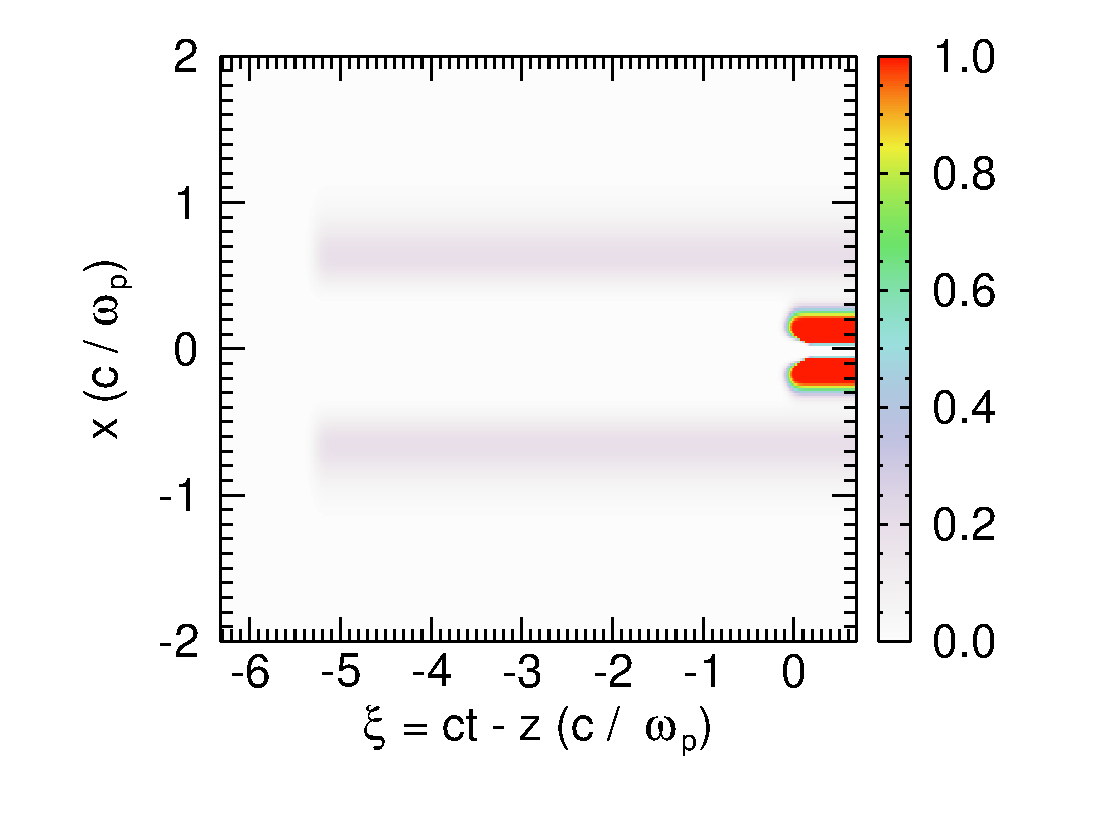
\includegraphics[width=.5\textwidth]{HICD.eps}
    }
    \\
        \subfloat[]{ 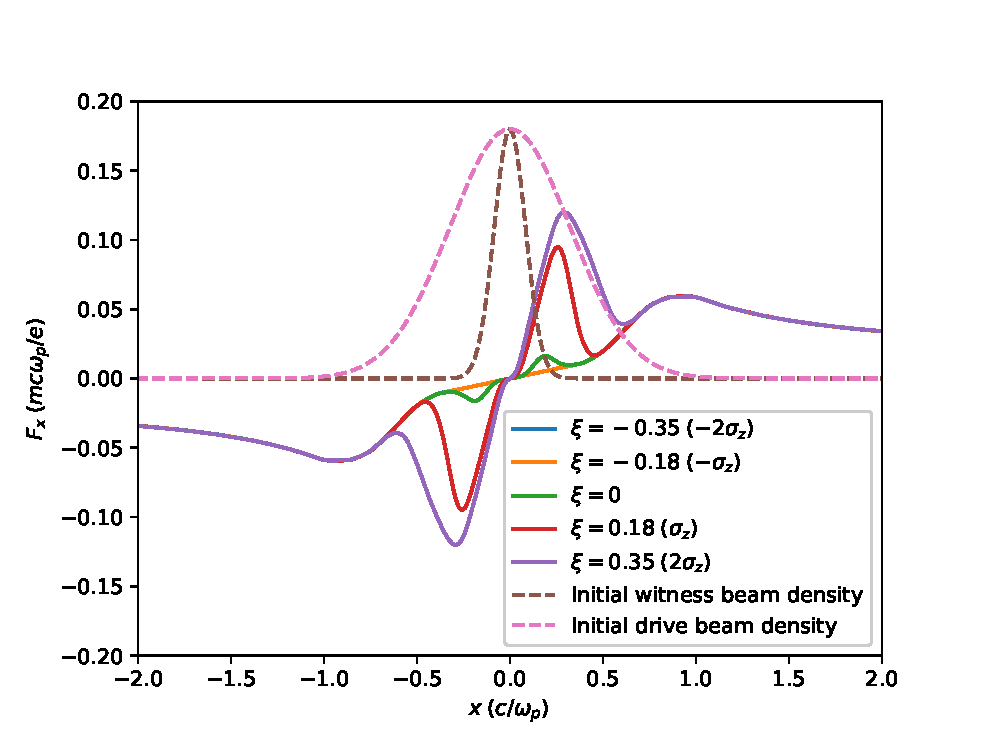
\includegraphics[width=.45\textwidth]{focus_x.eps}
        }
    \caption{(a) Helium ion charge density. The grey area is the
    helium ions produced by the drive beam, and the red area is the
    helium ions produced by the witness beam. (b) The $F_x$ transverse
    lineouts at different longitudinal positions, $\xi$, and the initial
    beam density profiles (in arbitrary units).} \label{fig:HICD_and_focus_x} \end{figure}

In order to avoid the emittance growth in the lithium plasma source, we
can increase the initial emittances for both the drive beam and witness beam.
In Fig. \ref{fig:he_buffer_emittance_growth}(b), we show the QuickPIC
simulation results when using an initial beam emittance of 20 $\mathrm{\mu m}$
 while keeping the other parameters the same as the
simulation shown in Fig. \ref{fig:he_buffer_emittance_growth}(a). When
the initial beam emittance becomes larger, the initial spot sizes of
both beams will increase, and the Coulomb field around the beam will
become smaller. Therefore, when the beams pass through the helium buffer gas,
the neutral helium is weakly ionized. However, the lithium can still
be ionized and form the plasma wake because lithium has a lower
ionization energy than helium. When there is no helium ionization, the
focusing force felt by the witness beam is linear, and its
emittance barely grows, as shown in
Fig. \ref{fig:he_buffer_emittance_growth}(b). The small emittance growth at the exit of the plasma in
Fig. \ref{fig:he_buffer_emittance_growth}(b) is still caused by the
helium ionization because the witness beam enters into the exit ramp of
helium with a smaller spot size compared to its initial spot size
at the entrance of the plasma.

\section{Conclusion} We have used theory and QuickPIC simulations to examine the evolution of the emittance and the Twiss parameters of particle beams in plasmas whose density is changing adiabatically. We use the WKB solution for each particle and assume the energy of each particle in the beam does not change
to obtain an analytical expression for the beam's emittance evolution in an
arbitrary adiabatic plasma density profile in a nonlinear PWFA. When the
beam has no initial energy spread, its emittance will remain a constant in the azimuthally symmetric  blowout regime.
When there is an initial energy spread, the beam's emittance can be
preserved as long as its initial Twiss parameters are matched to the density profile of the plasma
ramp. We also use this expression to analyze the emittance
growth when the position of the witness beam's focal plane in vacuum is changed while keeping the beam
parameters and the plasma density profile fixed. When the beam
cannot be matched, the emittance growth can be minimized by focusing the
unmatched beam to the same vacuum focal plane position as the matched
beam. We used QuickPIC simulations for 
possible FACET II beam parameters to show that the emittance can indeed be
preserved very well when we choose the focal plane position to be the same as
for a matched beam, even when the assumptions of symmetric blowout and adiabatic density evolution for the entire plasma region are not satisfied. 
%these simulation parameters don't quite satisfy the theoretical assumptions. 
For other focal
plane positions, the witness beam's emittance is larger at the exit
of the plasma. 
%In addition, we also examine through  simulations the effect of self-ionized plasmas when plasma is formed in a lithium gas that is contained by a helium buffer gas. When the drive 

In addition, we also examined through simulations the effect of additional self-ionization of the buffer gas by the drive beam. At FACET II a lithium gas is confined by a helium buffer gas. When the drive
and/or witness beam emittance is small (around 3 $\mathrm{\mu m}$), they can be focused to small enough spot sizes so that they can
ionize the helium buffer gas. This will lead to the focusing fields felt by the witness
beam to be strongly nonlinear. We find that this can potentially lead to the witness beam's emittance growing by a factor of 3 and 5 in the $x$ and $y$ planes respectively for sample FACET II parameters. The different growth in $x$ and $y$ directions is caused by the asymmetry of the
drive beam forming an asymmetric plasma wake. By using an initial
emittance of 20 $\mathrm{\mu m}$, the helium buffer gas is weakly
ionized and the witness beam's emittance can be preserved very well. 
% Put \label in argument of \section for cross-referencing
%\section{\label{}}
%
% If in two-column mode, this environment will change to single-column
% format so that long equations can be displayed. Use sparingly.
%\begin{widetext}
% put long equation here
%\end{widetext}
%
% figures should be put into the text as floats. Use the graphics or
% graphicx packages (distributed with LaTeX2e) and the \includegraphics
% macro defined in those packages. See the LaTeX Graphics Companion by
% Michel Goosens, Sebastian Rahtz, and Frank Mittelbach for instance.
% %
% Here is an example of the general form of a figure: Fill in the
% caption in the braces of the \caption{} command. Put the label that
% you will use with \ref{} command in the braces of the \label{}
% command. Use the figure* environment if the figure should span across
% the entire page. There is no need to do explicit centering.
% 
% \begin{figure} \includegraphics{TwoBunches.png}% \caption{\label{}}
% \end{figure}
% 
% 
% 
% 
% Surround figure environment with turnpage environment for landscape
% figure \begin{turnpage} \begin{figure} \includegraphics{}%
% \caption{\label{}} \end{figure} \end{turnpage}
% 
% tables should appear as floats within the text
% %
% Here is an example of the general form of a table: Fill in the caption
% in the braces of the \caption{} command. Put the label that you will
% use with \ref{} command in the braces of the \label{} command. Insert
% the column specifiers (l, r, c, d, etc.) in the empty braces of the
% \begin{tabular}{} command. The ruledtabular enviroment adds doubled
% rules to table and sets a reasonable default table settings. Use the
% table* environment to get a full-width table in two-column Add
% \usepackage{longtable} and the longtable (or longtable*} environment
% for nicely formatted long tables. Or use the the [H] placement option
% to break a long table (with less control than in longtable).
% \begin{table}%[H] add [H] placement to break table across pages
% \caption{\label{}} \begin{ruledtabular} \begin{tabular}{} Lines of
% table here ending with \\ \end{tabular} \end{ruledtabular} \end{table}
% 
% Surround table environment with turnpage environment for landscape
% table \begin{turnpage} \begin{table} \caption{\label{}}
% \begin{ruledtabular} \begin{tabular}{} \end{tabular}
% \end{ruledtabular} \end{table} \end{turnpage}
% 
% Specify following sections are appendices. Use \appendix* if there
% only one appendix.
\appendix \section{Calculation of beam moment $\braket{x^2}$}
%%% Appendix %%%
In this appendix we provide details on calculating the second moment of the beam, i.e., the square of the spotsize.
\[ \begin{aligned} \braket{x^2} &= \int x^2 f(x,x')dxdx' \\ &=\int x^2
f_i(x_i,x_i')dx_idx_i' \\ &= \int (M_{11}x_i + M_{12}x'_i)^2
f_i(x_i,x_i')dx_idx_i' \end{aligned} \] where $f(x,x')$ is the
distribution function at $z$ and $f_i$ is the initial distribution function. From
%Liouville's theorem 
the Vlasov equation 
we have $f(x,x') = f_i(x_i,x_i')$, and $dxdx' =
dx_idx_i'$ because det(M) = 1.

The last step above is correct only if all the particles have the same
energy. However, since different particles have different energy
$\gamma$, their corresponding transport matrices $M$ are different. In
order to calculate the above integral with an energy spread in the beam, we assume the main difference in
$M$ is the phase advance $\phi$. Even though the $\beta_m$, $\alpha_m$
in $M$ are different (because of different $\gamma$), we assume them to
be the same for all the particles and use $\gamma = \bar \gamma$ ($\bar
\gamma$ is the mean energy among all the particles), while claiming the
main difference is in $\phi$ due to different energy $\gamma$. After the beam propagates for a distance $z$, we
denote the distribution of
the phase advance $\phi$ as $f_{\phi}(\phi)$ (with the normalization
$\int f_{\phi}(\phi) d \phi=1$). So: 

\begin{equation} 
\begin{aligned} \braket{x^2}
&=\iiint (M_{11}x_i + M_{12}x'_i)^2 f(x_i,x_i')f_\phi(\phi)dx_idx_i'
d\phi \\ &= \braket{x_i^2} \int d\phi f_\phi(\phi) M_{11}^2 +
\braket{x_i'^2} \int d\phi f_\phi(\phi) M_{12}^2 \\ &\;\;\;\;+
\braket{x_i x_i'} \int d\phi f_\phi(\phi) 2M_{11}M_{12} \\ &=
\epsilon_i\Big[\beta_i \int d\phi f_\phi(\phi) M_{11}^2 + \gamma_i \int
d\phi f_\phi(\phi) M_{12}^2 \\ &\;\;\;\;-\alpha_i \int d\phi
f_\phi(\phi) 2M_{11}M_{12}\Big] \end{aligned} 
\end{equation}
where
\begin{equation} 
\begin{aligned}
&\int d\phi f_\phi(\phi) M_{11}^2 \\ &= \frac{\beta_m}{\beta_{mi}}
\int d\phi f_\phi(\phi) (\cos \phi + \alpha_{mi}\sin \phi)^2 \\ &=
\frac{1}{2}\frac{\beta_m}{\beta_{mi}}
[(1+C)+\alpha_{mi}^2(1-C)+2\alpha_{mi}S] \\ &=
\frac{1}{2}\frac{\beta_m}{\beta_{mi}}
[\beta_{mi}\gamma_{mi}+(1-\alpha_{mi}^2)C+2\alpha_{mi}S]
 \\ \\ 
 &\int
d\phi f_\phi(\phi) M_{12}^2 \\ &= \beta_m\beta_{mi} \int d\phi
f_\phi(\phi) \sin^2 \phi \\ &= \frac{1}{2}\beta_m\beta_{mi} (1-C) 
\\
\\ 
&\int d\phi f_\phi(\phi) 2M_{11}M_{12} \\ &= \beta_m \int d\phi
f_\phi(\phi) (2\cos \phi \sin \phi + 2\alpha_{mi} \sin^2\phi) \\ &=
\beta_m[S + \alpha_{mi}(1-C)] 
\end{aligned} 
\end{equation}
and where 
\begin{equation} 
C = \int d\phi f_\phi(\phi)\cos 2\phi, \;\; S = \int d\phi f_\phi(\phi)\sin 2\phi
\end{equation}
Finally, we obtain: 
\begin{equation} 
\begin{aligned} \braket{x^2} &=\epsilon_i \beta_m\Big[ \frac{\beta_i
\gamma_{mi}+\gamma_i \beta_{mi}-2\alpha_i \alpha_{mi}}{2} \\
&\;\;\;+(\frac{\beta_i}{\beta_{mi}}-\frac{\beta_i
\gamma_{mi}+\gamma_i\beta_{mi}+2\alpha_i\alpha_{mi}}{2})C \\
&\;\;\;+(\frac{\beta_i}{\beta_{mi}}\alpha_{mi}-\alpha_i)S\Big]
\end{aligned} 
\end{equation}
 We can define: 
\begin{equation} 
\begin{aligned} A &= \frac{\beta_i
\gamma_{mi}+\gamma_i \beta_{mi}-2\alpha_i \alpha_{mi}}{2} \\ B_1 &=
\frac{\beta_i}{\beta_{mi}} - A = \frac{\beta_i}{\beta_{mi}}
-\frac{\beta_i \gamma_{mi}+\gamma_i \beta_{mi}-2\alpha_i \alpha_{mi}}{2}
\\ B_2 &= \frac{\beta_i}{\beta_{mi}}\alpha_{mi}-\alpha_i \end{aligned} 
\end{equation}
Leading to: \begin{equation} \braket{x^2} = \epsilon_i\beta_m(A + B_1 C +
B_2 S) \end{equation}

\section{Proof of $A \geqslant 1$} 
\begin{equation} \begin{aligned}
A &= \frac{\beta_i \gamma_{mi}+\gamma_i \beta_{mi}-2\alpha_i
\alpha_{mi}}{2} \\ & \geqslant \frac{2\sqrt{\beta_i \gamma_{mi}\gamma_i
\beta_{mi}}-2\alpha_i \alpha_{mi}}{2} \\ &=
\sqrt{(1+\alpha_i^2)(1+\alpha_{mi}^2)}-\alpha_i \alpha_{mi} \\ &=
\sqrt{1+\alpha_i^2 +\alpha_{mi}^2+ \alpha_i^2\alpha_{mi}^2 }-\alpha_i
\alpha_{mi} \\ & \geqslant \sqrt{1+2\alpha_i \alpha_{mi}+
\alpha_i^2\alpha_{mi}^2 }-\alpha_i \alpha_{mi} \\ & = |1+\alpha_i
\alpha_{mi} | -\alpha_i \alpha_{mi} \\ & \geqslant 1 \end{aligned}
\end{equation}

\section{}
In this appendix we derive the first order correction to the phase advance due to variation of the energy of the particle. We begin with the definition for the phase
\[
\phi = \int_0^z \frac{\omega_p(s)}{\sqrt{2  \gamma}c} ds
\]
Due to the variation of $\gamma$, the variation of $\phi$ is
\begin{equation}
\begin{aligned}
\Delta \phi 
&= \Delta \int_0^z \frac{\omega_p(s)}{\sqrt{2  \gamma}c} ds
\\
& = \int_0^z \Delta(\frac{\omega_p(s)}{\sqrt{2  \gamma}c}) ds
\\
&= \int_0^z -\frac{1}{2}(\frac{\omega_p(s)}{\sqrt{2}\gamma^{\frac{3}{2}}c}) \Delta \gamma ds
\\
&= -\frac{\Delta \gamma}{2\gamma}\int_0^z \frac{\omega_p(s)}{\sqrt{2\gamma}c} ds
\\
&= -\frac{\phi}{2\gamma}\Delta \gamma
\end{aligned}
\end{equation}
So the difference between the phase advance of a particle with energy $\gamma$ and the phase advance of a particle with the average energy $\bar \gamma$ is
\begin{equation}
\begin{aligned}
\phi(\gamma) - \phi(\bar \gamma) = -\frac{\phi(\bar \gamma)}{2\bar \gamma} \Delta \gamma
\end{aligned}
\end{equation}
and
\begin{equation}
\begin{aligned}
\phi(\gamma) = \bar \phi -\frac{\bar \phi}{2\bar \gamma} \Delta \gamma
\end{aligned}
\end{equation}

\section{Differential equation for $\beta$}
In this appendix, we offer a derivation of equation (\ref{ODE})  in the text.
We start from the definition of the beam's spot size:
\[
	\sigma_x = \sqrt{\braket{x^2}}
\]
Taking derivatives with respect to $z$ provide:
\[
	 \sigma_x' = \frac{\braket{xx'}}{\sigma_x}
\]
\[
	\sigma_x'' = \frac{\braket{x^2}\braket{x'^2} - \braket{xx'}^2}{\sigma_x^3} + \frac{\braket{xx''}}{\sigma_x}
\]
 Using the definition of geometric emittance (\ref{geoEmittanceDef}) and the equation of motion (\ref{EOM}), leads to:
 \[
 	\sigma_x'' = \frac{\epsilon^2}{\sigma_x^3} - k_\beta^2 \sigma_x
 \]
If we assume the beam has no energy spread, then under a linear focusing force, the beam's normalized emittance $\epsilon_n$ is a constant, so $\epsilon = \epsilon_n / \gamma$ is also a constant. Finally, if we use the definition of $\beta$: $\beta = \frac{\sigma_x^2}{\epsilon}$, we obtain
\[
\frac{1}{2} \beta \beta'' -\frac{1}{4} \beta'^2 + \beta^2 k_\beta^2 = 1
\]
%%% Appendix %%%
% If you have acknowledgments, this puts in the proper section head.
\begin{acknowledgments} This work was supported by the U.S. Department of
Energy under Grants No. DE-SC0010064, and SCIDAC under Grants No. 644405, and the National Science Foundation under Grants No. 1806046. The simulations were run on Bluewaters, NERSC, and the UCLA Hoffman2 clusters. \end{acknowledgments}
% Create the reference section using BibTeX:
%\bibliographystyle{IEEEtran} \bibliographystyle{plainnat}
\bibliography{reference}
\end{document}
%
% ****** End of file apstemplate.tex ******
% 
